%\part{Aspectos Gerais}

\chapter[Referencial Teórico]{Referencial teórico}
	
	Este capítulo tem como objetivo servir como referencial teórico para todo o documento. Inicialmente o capítulo apresenta uma visão geral sobre o processo de contratação de software na APF, destacam-se a importancia de algumas leis que servem como fundamento para a contratacao de terceirizadas e o nível de qualidade que é exigido por parte dos orgãos públicos. Em seguida discute-se sobre o conceito de qualidade de software na visão de alguns atores e o que é qualidade segundo a ISO 9126 que serviu como base para a norma SQUARE também discutida neste trabalho. Após a definição de qualidade pela norma SQUARE, é apresentado conceitos fundamentais de manutenção de software que servem como guia para o desenvolvimento deste trabalho. Tendo definido manutenabilidade alguns conjuntos de métricas que visam identificar possíveis lacunas de manutenabilidade no código são apresentados. Com as métricas definidas é necessário que se faça a devida visualização das métricas, tópico final deste capítulo.
	
\section{Processo de Contratação de Software na APF}
O Decreto n\c 2.271 de 1997 \cite{decreto_2271} dispõe sobre a contratação de serviços pela APF. Segundo o Decreto todos os produtos ou serviços que não apresentam relação direta com o propósito da instituição do governo federal devem ser tercerizados. O Decreto coloca como exemplo algumas atividades como por exemplo, conservação, limpeza, segurança, vigilância, transportes, informática, copeiragem, recepção, reprografia, telecomunicações são atividades livres para tercerização.
\\A licitação é um conjunto de processos administrativos de caráter formal para as compras de bens ou serviços nos governos federais, estaduais ou municipais. Segundo a Lei  n 8.666 de 1993, o governo brasileiro para garantir a isonomia (princípio geral do direito segundo o qual todos são iguais perante a lei) diz que para contratações de bens ou serviços deve-se dar prioridade para licitação \cite{Lei_1993}. A licitação pode ocorrer de quatro categorias: concorrência, tomada de preços, convite e pregão \cite{brazil_licitacoes_2010}.
\\Uma vez que uma empresa ganha a licitação para um serviço a empresa ganha o direito de contratação para prestar o serviço ao orgão contratante. Para ajudar no processo de contratação de empresas terceirizadas voltadas para a área de TI o TCU disponibiliza um Guia de boas práticas de contratações em soluções de TI \cite{guia_boas_praticas}. Segundo o guia a prática de contratação do serviço de desenvolvimento de um sistema de informação pode englobar elementos do tipo:
\begin{itemize}
\item Os softwares do sistema, devidamente documentados e com evidências de que foram testados;
\item As bases de dados do sistema, devidamente documentadas;
\item O sistema implantado no ambiente de produção do órgão;
\item A tecnologia do sistema transferida para a equipe do órgão, que deve ocorrer ao longo de todo o contrato;
\item As rotinas de produção do sistema, devidamente documentadas e implantadas no ambiente de produção do órgão;
\item As minutas dos normativos que legitimem os atos praticados por intermédio do sistema;
\item O sistema de indicadores de desempenho do sistema implantado, que pode incluir as atividades de coleta de dados para gerar os indicadores, fórmula de cálculo de cada indicador e forma de publicação dos indicadores. Citam-se, como exemplos, os indicadores de disponibilidade, de desempenho das transações e de satisfação dos usuários com o sistema de informação;
\item Os scripts necessários para prover os atendimentos relativos ao sistema por parte da equipe de atendimento aos usuários, devidamente implantados e documentados;
\item A capacitação dos diversos atores envolvidos com o sistema (e.g. equipe de suporte técnico do órgão, equipe de atendimento aos usuários, equipe da unidade gestora do sistema e usuários finais), que pode envolver treinamentos presenciais e a distância;
\item O serviço contínuo de suporte técnico ao sistema (e.g. atendimento aos chamados feitos pelo órgão junto à contratada sobre dúvidas e problemas relativos ao sistema);
\item O serviço contínuo de manutenção do sistema (e.g. implantação de manutenções corretivas e evolutivas).
\end{itemize} 
Tendo definido o que pode ser terceirizado dentro de um órgão público, é necessário que o produto entregue tenha qualidade aceitável para que seja fechado o acordo por parte da tercerizada e da contratante (neste caso APF). Contudo é necessário estipular o que é avaliado durante a contratação de um software.

\subsection{Avaliação da Qualidade Em Um Processo de Contratação }
Uma vez que o software é produzido pela tercerizada o software passa por um processo de verificação de todo o artefato que foi entregue seja ele em forma de código, como em forma de documentos. São lançados dezenas de editais todos os anos com o intuito de suprir a necessidade dos órgãos públicos quanto a demanda de software. Cada órgão é responsável por disponibilizar o seu edital contendo entre vários assuntos a forma como será inspecionado o código entregue pela tercerizada. Em um edital feito pelo DNPM \cite{edital} um dos objetos de avaliação é a cobertura miníma de testes como mostra a Tabela \ref{tabela1}, são avaliados tanto testes unitários, como de interface e de integração.

\begin{table}[h]
\centering
\caption{Índice de Cobertura Por Tipo de Teste do Edital da DNPM. Fonte:\cite{edital}}
\label{tabela1}
\begin{tabular}{ll}
\textbf{Tipo de Teste} & \textbf{\% de cobertura} \\
Unitários              & 70\%                     \\
De Integração          & 100\%                    \\
De Interface           & 20\%                    
\end{tabular}
\end{table}

Este mesmo edital também apresenta outra tabela \ref{tabela2} mostrando outros detalhes que também serão cobrados na entrega do software. Algumas características desta tabela devem ser salientadas, como por exemplo, algumas métricas (mais especificamente taxa de cobertura de código, complexidade por método e LCOM4) não possuem valores definidos de cobrança e são ajustados de acordo com o projeto.
\begin{table}[h]
\centering
\caption{Métricas de Qualidade de Código Exigidas pela DNPM. Fonte: \cite{edital}}
\label{tabela2}
\begin{tabular}{|l|l|l|}
\hline
\textbf{Métrica}                      & \textbf{Meta}                                                                                                   & \textbf{Severidade} \\ \hline
Taxa de cobertura de código          & Definida na Demanda                                                                                             & Média              \\ \hline
Complexidade por método              & Definida na Demanda                                                                                             & Média              \\ \hline
Coesão (LCOM4)                       & Definida na Demanda                                                                                             & Média              \\ \hline
Violações do tipo Blocker           & Zero                                                                                                            & Média               \\ \hline
Violações do tipo Critical          & Zero                                                                                                            & Média               \\ \hline
Violações do tipo Major             & \begin{tabular}[c]{@{}l@{}}Igual ou menor que 0,5\% em\\ relação ao total de linhas de\\ código\end{tabular} & Baixa               \\ \hline
Violações do tipo Minor             & \begin{tabular}[c]{@{}l@{}}Igual ou menor que 1\% em\\ relação ao total de linhas de\\ código\end{tabular}   & Baixa               \\ \hline
Taxa de sucesso em testes unitários  & 100\%                                                                                                           & Baixa               \\ \hline
Taxa de duplicações de blocos       & Igual ou menor que 2\%                                                                                          & Baixa               \\ \hline
Taxas de comentários da API Pública & Maior ou igual a 80\%                                                                                           & Baixa               \\ \hline
Linhas de código comentadas          & \begin{tabular}[c]{@{}l@{}}Igual ou menor que 0,1\% em\\ relação ao total de linhas de\\ código\end{tabular} & Baixa               \\ \hline
\end{tabular}
\end{table}

\section{Qualidade}
	O principal produto da engenharia de software é o software, contudo o que tem se vivenciado na realidade brasileira de computação é que o software que está sendo entregue é um software precário e de baixa qualidade. Por ser uma palavra abstrata, o conceito de qualidade é bem amplo, porém o termo qualidade normalmente está associado a uma medida relativa, essa qualidade pode ser entendida como "conformidade às especificações". Conceituando dessa forma, a não conformidade às especificação é igual a ausência de qualidade \cite{Paduelli}.
\\ A ISO 9126-1 proposta em 2001, também conhecida como Engenharia de Software - Qualidade do Produto, descreve o modelo de qualidade voltado para o produto de software como sendo composto por duas categorias como pode ser visto na Figura \ref{img:relacao_iso}. A primeira categoria está relacionada a qualidade interna e a qualidade externa do software. A segunda categoria se relaciona com a qualidade de uso do software \cite{_nbr_2016}
\graphicspath{{figuras/}}
\begin{figure}[h]
\centering
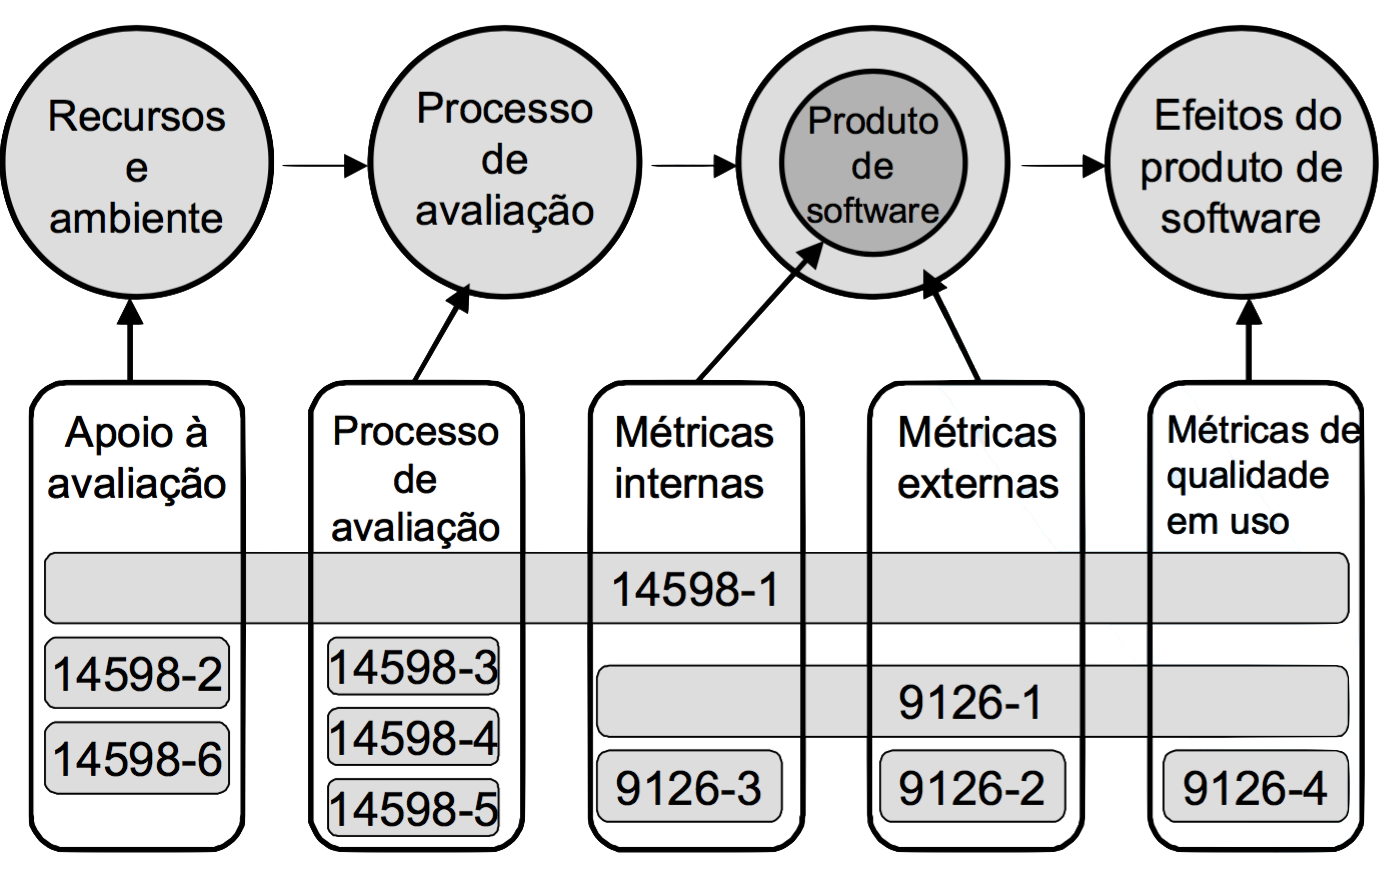
\includegraphics[scale=0.40]{ISO}
\caption{Relação entre as NBR ISO/IEC 9126 e NBR ISO/IEC 14598 .Fonte:\cite{_nbr_2016}}
\label{img:relacao_iso}
\end{figure}
\\ Sob o aspecto de modelo de qualidade,a ISO 9126 classifica a qualidade interna do produto como sendo o somatório das características do ponto de vista interno do software. Os principais produtos desta categoria são os de cunho intermediário, entre eles: relatórios de analise estática do código fonte, revisão dos documentos produzidos, entre outros. A qualidade externa por sua vez já apresenta o seu foco mais voltado para as relações externas do software, normalmente esta relacionado com a execução do código coletando suas métricas enquanto o software está em funcionamento. A Figura \ref{img:modelo_qualidade} apresenta a divisão proposta pela \cite{_nbr_2016} onde são categorizados seis aspectos de qualidade de software e suas subcaracterísticas, essas podem ser medidas por meio de métricas internas e externas. 
\graphicspath{{figuras/}}
\begin{figure}[h]
\centering
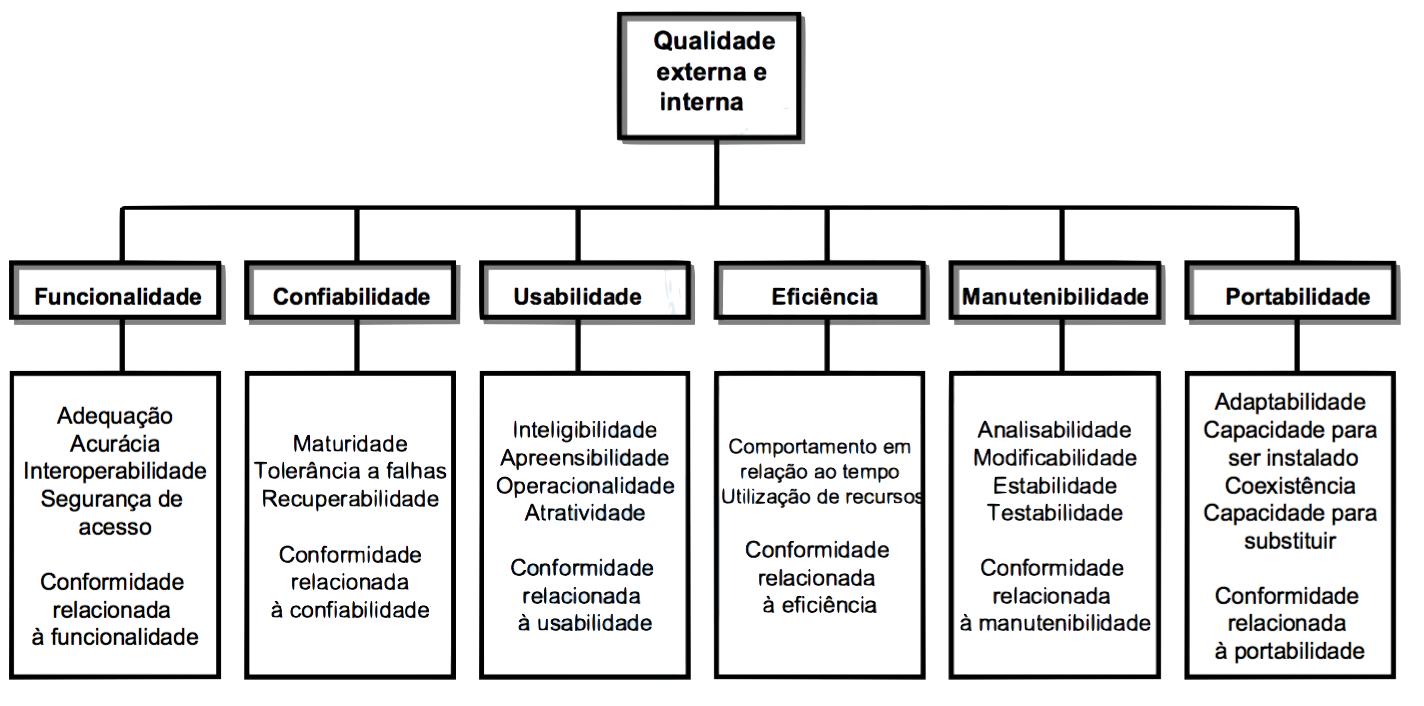
\includegraphics[scale=0.50]{Modelo_de_Qualidade}
\caption{Modelo de Qualidade para Qualidade Interna e Externa .Fonte:\cite{_nbr_2016}}
\label{img:modelo_qualidade}
\end{figure}
\\Segundo a ISO 9126 essas caracteristicas podem ser definidas como:
\begin{itemize}
\item \textbf{Funcionalidade}: Capacidade do produto de software de prover funções que atendam às necessidades explícitas e implícitas, quando o software estiver sendo utilizado sob condições especificadas.
\item \textbf{Confiabilidade}:Capacidade do produto de software de manter um nível de desempenho especificado, quando usado em condições especificadas.
\item \textbf{Usabilidade}: Capacidade do produto de software de ser compreendido, aprendido, operado e atraente ao usuário, quando usado sob condições especificadas.
\item \textbf{Eficiência}: Capacidade do produto de software de apresentar desempenho apropriado, relativo à quantidade de recursos usados, sob condições especificadas.
\item \textbf{Manutenibilidade}: Capacidade do produto de software de ser modificado. As modificações podem incluir correções, melhorias ou adaptações do software devido a mudanças no ambiente e nos seus requisitos ou especificações funcionais.
\item \textbf{Portabilidade}: Capacidade do produto de software de ser transferido de um ambiente para outro.
\end{itemize}
Em 2011 surgiu um conjunto de normas conhecidos como SQuaRE que traziam um framework aprimorado à atual norma vigente. Este framework tinha como objetivo avaliar o produto de qualidade de software.

\subsection{Norma SQuaRE}
O conjunto de normas SQuaRE (Requisitos e Avaliação de Qualidade de Sistema e Software) surgiu para substituir a ISO/IEC 9126. O objetivo destas normas é prover um framework que avalie a qualidade do produto de software \cite{luiza_yago}. ISO/IEC 25010 mantém as características de qualidade já definidas na ISO 9126 com alguns incrementos.

\begin{itemize}
\item O escopo dos modelos de qualidade foram extendidos para incluir sistemas computacionais e a qualidade em uso pelo ponto de vista do sistema
\item Segurança foi adicionada como característica, e não uma subcaracterística de funcionalidade.
\item Compatibilidade foi adicionada como característica.
\item A qualidade interna e externa foram combinadas como modelo de qualidade de produto.
\end{itemize}

A norma apresenta três guias de qualidade. O primeiro modelo é referente à Qualidade do Produto, o segundo da Qualidade em Uso e o último Qualidade de Dados.O modelo de Qualidade do Produto subdivide um sistema de software em oito categorias como mostra a imagem \ref{img:modelo_square}.
Assim como a ISO 9126, a ISO 25010 também apresenta categorias, estas categorias se assemelham às categorias da ISO 9126 a qual serviu como base para criação da norma SQuaRE, estas caracteristicas são:

\begin{itemize}
\item \textbf{Adequação Funcional}: nível que determina o quanto um produto ou sistema satisfazem as especificações providas pelo usuário.
\item \textbf{Eficiência de Performance}: performance relativa à quantidade de recursos usados em condições específicas.
\item \textbf{Compatibilidade}: o nível que um sistema ou produto pode compartilhar informaçõesc com outros produtos, sistemas ou componentes.
\item \textbf{Usabilidade}: O nível que um produto ou sistema pode ser usado por usuários específicos para atingir seus objetivos com efetividade, eficiência e satisfação em contexto específico de uso.
\item \textbf{Confiabilidade}: nível que um sistema, produto ou componente executa suas atividades em um contexto pré-determinado e específico para uso.
\item \textbf{Segurança}: nível no qual um sistema protege as informações e os dados de maneira que pessoas ou outros sistemas tenham acesso limitado de acordo com nível de autorização especifíco.
\item \textbf{Manutenibilidade}: nível de efetividade e eficiência com o qual um produto ou sistema pode ser modificado pelos sistemas mantenedores.
\item \textbf{Portabilidade}: Nível de efetividade e eficiência com o qual um sistema, produto ou componente pode ser transferido de um hardware, software ou ambiente de uso para outro.
\end{itemize}

\graphicspath{{figuras/}}
\begin{figure}[h]
\centering
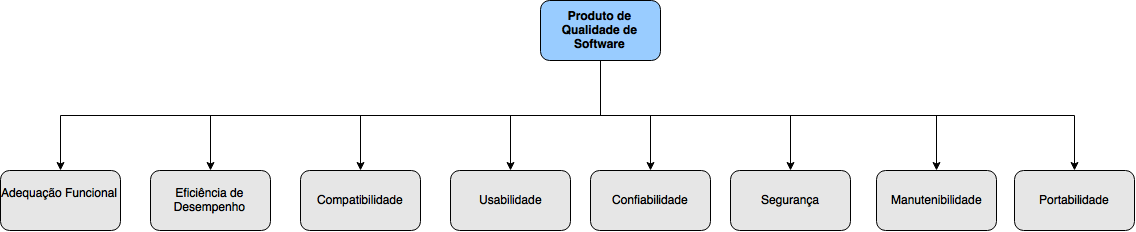
\includegraphics[scale=0.40]{SQuaRE}
\caption{Produto de Qualidade de Software.Fonte:\cite{Square}}
\label{img:modelo_square}
\end{figure}

Este trabalho tem seu desenvolvimento focado no modelo de Qualidade de Uso que apresenta características externas ao software e os resultados são coletados através de atributos estáticos \cite{Square}. O foco deste trabalho está em medir indicadores quanto à manutenabilidade do software. Essa característica está diretamente ligada ao processo de Manutenção do Software.  

\subsection{Manutenção de Software}
Segundo Sommervile \cite{sommervile} manutenção de software é o processo de alterar o sistema depois que ele foi publicado. As alterações feitas no software podem ser simples correções de erro, a até mudanças significativamente grandes que corrigem falhas arquiteturais, ou mesmo melhorias para acomodar novos requisitos.
\\Outra visão sobre manutenção de software é dada por Pressman \cite{pressman} em que o autor conceitua o termo como sendo a correção de defeitos, adaptação do software para atender uma mudança do ambiente e aperfeiçoar as funcionalidades para que atendam às necessidades dos usuários. Outra característica do processo de manutenção é a sua composição por um conjunto de sub processos, atividades e tarefas que podem ser utilizados durante a fase de manutenção para alterar um produto de software, contanto que seja mantido o seu funcionamento \cite{calazans_avaliacao_2005}.
\\Para Sommervile existem quatro categorias de manutenção:
\begin{itemize}
\item \textbf{Manutenção Corretiva}: seu objetivo está em identificar e remover falhas de software
\item \textbf{Manutenção Adaptativa}: provê modificações no software para alojar mudanças no ambiente externo. Nesta manutenção também está incluso o processo de migração para diferentes plataformas tanto de software quanto de hardware.
\item \textbf{Manutenção Perfectiva}: está manutenção é feito com o intuito de aperfeiçoar o software, além dos requisitos funcionais originais. Esta expansão dos requisitos traz consigo uma melhoria às funcionalidades até então implementadas ou um ganho de performance do sistema.
\item \textbf{Manutenção Preventiva}: implementada para permitir que seja mais simples a correção, adaptação ou melhoria do software.
\end{itemize}

O modelo da figura \ref{img:modelo_manutencao} apresenta as atividades propostas por Pfleeger para um processo de manutenção. Na figura percebe-se que o processo de acompanhamento da manutenção ocorre durante todo o processo. As atividades apresentadas no diagrama são:

\begin{itemize}
\item \textbf{Analise do Impacto da Mudanção de Software}: estima o impacto de uma determinada mudança. Nesta atividade determina-se o grau de mudança e o quanto está mudança impactará no resto do software. 
\item \textbf{Entendimento do Software a ser Alterado}: nesta atividade são analisados os códigos-fonte do software para entender a mudança e a integração do que deve ser alterado. Esta atividade depende muito do grau de manutenabilidade do software, uma vez que quanto mais manutenível mais fácil e rapido se dá o processo de analise do software.
\item \textbf{Implementação da Mudança}: incremento ou modificação do software. Está atividade é diretamente relacionada com o grau de adaptação do software, o quanto o software pode ser expandido ou comprimido. Essa característica de adaptabilidade é uma subcaracterística da Manutenabilidade de software apresentada pela norma Square. 
\item \textbf{Mudanças pelo Efeito Cascata}: Analise da propagação das mudanças ao longo do software. Essa atividade está intimamente relacionada com o indicador de coesão e acomplamento do software, este afere o quão amarrado estão as classes e os métodos do software.
\item \textbf{(Re)Teste do Software}: é a ultima atividade antes da entrega do software alterado. O software é testado novamente sob a perspectiva do novo requisito.
\end{itemize}

\graphicspath{{figuras/}}
\begin{figure}[h]
\centering
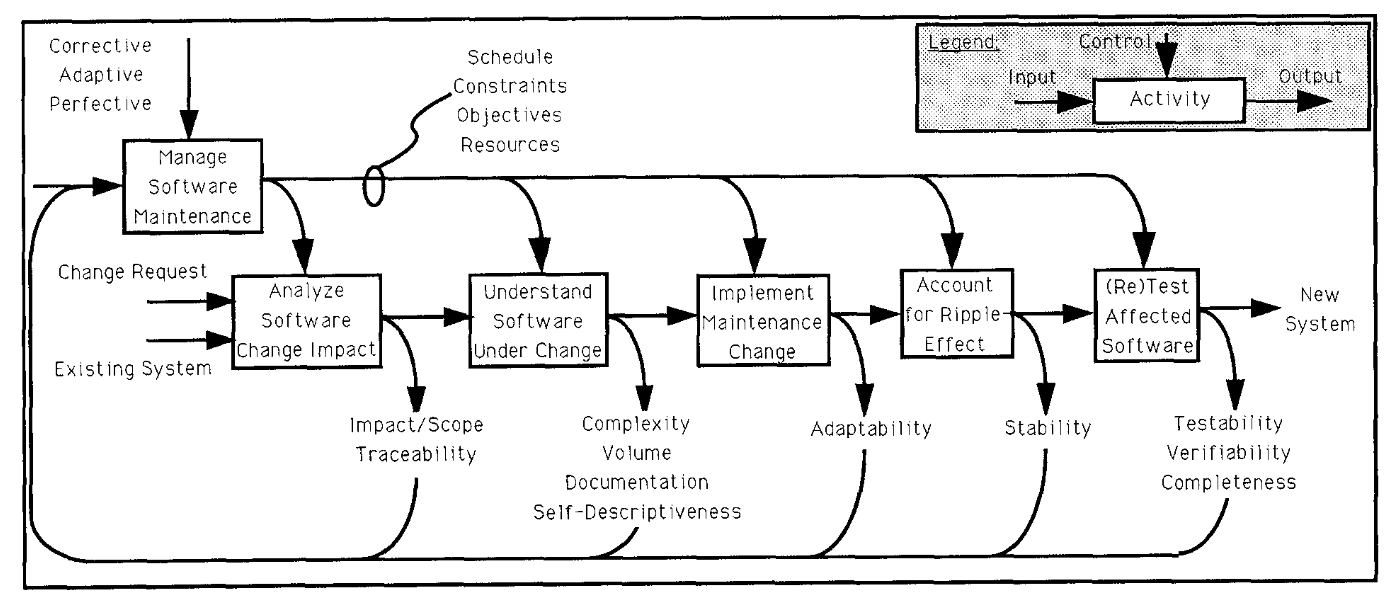
\includegraphics[scale=0.50]{Manutencao}
\caption{Diagrama das Atividades de Manutenção de Software.Fonte:\cite{pfleeger_framework_1990}}
\label{img:modelo_manutencao}
\end{figure}
Um estudo realizado por Kustyers e Heemstra \cite{kusters} mostram a dificuldade de atuais na manutenção de software em seis grandes organizações da Alemanha. Um dos resultados obtidos foi que existe um uma falta muito grande na percepção quanto ao tamanho e o custo das manutenções de software. Os autores relatam que os gastos com manutenção são altos e que das seis empresas apenas uma mantinha registrado os seus processos de manutenção e os usava para fazer um novo planejamento. 
\\Normalmente tem se como verdade de que a manutenção de software está unicamente ligada ao conserto de \textit{bugs}, entretanto estudos e \textit{surveys} ao longo dos anos comprovam que mais de 80\% do esforço gasto na manutenção é utilizado em ações não corretivas segundo Pigosky \cite{pigosky}. O autor também afirma que entre 40\% a 60\% do esforço de manutenção está em entender o software que será modificado.

\section{Métricas de Qualidade de Software}
Uma métrica é uma função que pode ser medida, e métrica de qualidade de software é uma funcão na cuja entrada é uma informação de software e cuja saida é um único valor numérico que pode ser interpretado como nível que é dado a um software \cite{karner}. Segundo \cite{pressman} métricas podem ser definidas como sendo um pequeno subconjunto de informações que tem informações úteis acerca do software.
Segundo Mills algumas características são inerentes a uma boa métrica, caracteristicas como, simplicidade,objetividade, fácil obtenção, validade, robustez, linearidade de escala. Diversos autores sugeriram conjunto de métricas que combinadas tratam de várias áreas de qualidade de software \cite{paulo_meirelles}.

\subsection{Suíte de Chidamber-Kemerer}
Este conjunto de métricas foi proposto por Shyam R. Chidamber e por Chris F. Kemerer em 1994 tem como objetivo avaliar aspectos de qualidade interna dos artefatos produzidos sob a visão de uma linguagem orientada a objetos \cite{chidamber}. A suíte apresenta as seguintes métricas:
\begin{itemize}

\item \textbf{WMC}: Em uma classe com \textit{n} métodos, a complexidade é dada como sendo a complexidade dos \textit{n} métodos. 
 \begin{equation}
WMC = \sum_{i=1}^{n}Ci
\end{equation}


Essa métrica serve como indicador para o nível geral da modularização. Quanto maior o valor mais complexas estão a classe ou poucas classes possuem um indíce de complexidade muito alto.

\item \textbf{DIT}: Tamanho do maior caminho entre a raiz da árvore de herança e a classe a qual está sendo analisada. Essa métrica permite ver o quanto uma mudança em uma determinada classe pode afetar todo o sistema.

\item \textbf{NOC}: Quantidade de classes que se utilizam da classe em analise, seja por herança ou implementação. Essa métrica junto com outras ajuda a determinar quais classes são primordiais para o funcionamento do sistema.

\item \textbf{CBO}: Está métrica é dada pela equação 2.2: 

\begin{equation}
CBO = \frac{NumberOfDependencies}{NumberOfClassInPackage}
\end{equation}
Uma dependência pode ser definida como o uso de um método ou variável de outra classe porém do mesmo pacote.

\item \textbf{RFC}: Número de métodos e construtores distintos que são chamados por uma classe. Está medida é muito utilizada para cobertura de testes, em que é pode ser constatado a necessidade ou não de uma modularização de uma classe.

\item \textbf{LCOM}: Sendo \textit{C} uma classe com \textit{n} métodos, seja \textit{In} o conjunto de variáveis de instância utilizadas pelo método \textit{n}, seja \textit{P} o conjunto tal que:
\begin{equation}
P = \{(Ii,Ij)|(Ii\bigcap Ij)= \o\}
\end{equation}
e \textit{Q} o conjunto tal que:
\begin{equation}
Q = \{(Ii,Ij)|(Ii\bigcap Ij)= \o\}
\end{equation}
então LCOM é definida como sendo:
\begin{equation}
LCOM = |P| - |Q| se |P|>|Q|
\end{equation}
ou zero caso contrário.
\end{itemize}

\subsection{Suíte MOOD}
Outro conjunto de métricas que tem como objetivo de medir de maneira quantitativa é a suíte de métricas MOOD. Ela conta com oito métricas. Essas métricas visam atender as principais características da orientação a objeto, então principios como polimorfismo, baixo acoplamento, encapsulamento e outros princípios são altamente valorizados. As métricas são \cite{paulo_meirelles} \cite{moreira_avaliacao_2015}
\begin{itemize}
\item \textbf{MHF}: Métrica que indica a razão entre a soma de todos os métodos que são invisíveis em relação ao total de métodos do sistema.
\\Número de métodos Visíveis em uma classe C
\begin{equation}
Mv(C)
\end{equation}
\\Número de métodos encapsulados em uma classe C
\begin{equation}
Me(C)
\end{equation}
\\O total de métodos é dado por
\begin{equation}
Mt(C) = Mv(C)+Me(C)
\end{equation}
\\A equação que representa esta métrica é dada por:
\begin{equation}
MHF =\frac{\sum_{TC}^{i=1}Mh(Ci)}{\sum_{TC}^{i=1}Mt(Ci)}
\end{equation}
Onde TC é o total de classes analisadas.

\item \textbf{AHF}: Razão do somatório de todas os atributos que são herdados de todas as classes em relação ao número total de atributos. A equação que descreve este método é semelhante a dada por MHF
\begin{equation}
AHF =\frac{\sum_{TC}^{i=1}Ah(Ci)}{\sum_{TC}^{i=1}At(Ci)}
\end{equation}

\item \textbf{MIF}: Razão entre o somatório dos métodos herdados nas classes e o número total de métodos presentes no sistema.
\begin{equation}
MIF = \frac{TMh}{TMd}
\end{equation}
\item \textbf{AIF}: Razão entre a soma dos atributos herdados em todas as classes do sistema e o total de atributos da classe.
\begin{equation}
MIF = \frac{TAh}{TAd}
\end{equation}
\item \textbf{CFA}:Razão entre o total de acomplamentos permitídos no sistema e o atual número de acoplamentos possíveis por herança. Para está metrica toma-se como base uma relação cliente servidor entre as classes. Sempre que existir uma referência a um método ou atributo da classe servidora, usa-se a seguinte equação para calcular o fator de acoplamento.
\begin{equation}
COF = \frac{\sum_{TC}^{i=1}[\sum_{TC}^{i=1}isClient(Ci,Cj)]}{TC^2-TC}
\end{equation}
\item \textbf{PFA}: Razão entre o numéro atual de possibilidades de polimorfismo diferentes que podem ser utilizados em uma classe e o número máximo de polimorfismos diferentes que podem haver nesta mesma classe.
\end{itemize}

Uma vez que as métricas se encontram definidas, deve-se pensar na melhor maneira de exibir as métricas para o usúario. O papel da visualização das métricas de software é definir com base na natureza, e na escala de uma métrica qual a melhor maneira de imprimir na tela essas informações.

\section{Visualização da Informação}
Computadores se tornaram peças fundamentais cotidiano do ser humano do século 21. Seja para lazer, estudo, comunicação, o computador revolucionou significamente em cada área que passou \cite{hasan_humancomputer_2014}.
A visualização de software pode ser definida como uma disciplina que faz uso de várias formas de imagens que servem de insumo para compreender, entender e reduzir a complexidade dos sistemas de software existentes \cite{gracanin_software_2005}. Porém a visão que melhor se adapta ao contexto deste trabalho é dada por Gomes \cite{gomes_percepcao_2011} que diz que a visualização de uma forma generalizada é a construção de uma imagem visual na mente humana e está imagem vai além de representações gráficas ou conceitos.



\subsection{Visualização de Dados}
Segundo Gomes \cite{gomes_percepcao_2011} algumas técnicas para visualização de dados são mais eficazes do que outras dependendo da natureza do dado a ser observado. Gomes destaca duas técnicas de visualização de dados.

\begin{itemize}
\item \textbf{Visualização de Atributos}: Nesta técnica a natureza do dado é representado através de um gráfico ou um mapa. Também é possível representar através de ícones ou \textit{glifos}. ícones normalmente representam uma entidade ou um elemento que pertence a um contexto. O \textit{glifo} representa um objeto geométrico que representa uma entidade ou um elemento do todo. O \textit{glifo} tem uma forma que é definida pelo valor dos atributos da entidade como pode ser visto na figura \ref{img:glifo}.
\graphicspath{{figuras/}}
\begin{figure}[h]
\centering
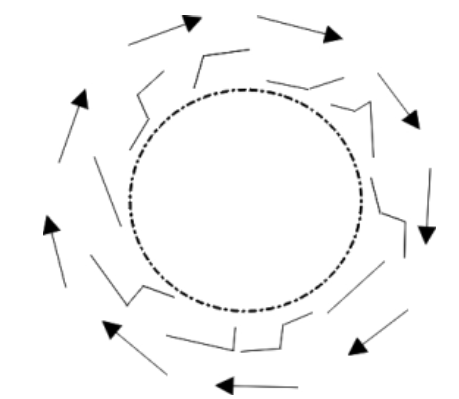
\includegraphics[scale=0.5]{Glifo}
\caption{Exemplo de glifo utilizado na visualização da variação das medidas relacionadas com o desenvolvimento computacional. Fonte: \cite{gomes_percepcao_2011}}
\label{img:glifo}
\end{figure}

\item \textbf{Visualização de Estruturas e Relações}: está técnica utiliza do conjunto de dados ou elementos que podem ser distribuitos de maneira hierarquica. Dentro deste conceito existe uma ramificação para o uso da técnica aplicado de maneiras diferentes que possuem focos diferentes, algumas dessas técnicas são \textit{Bifocal Display} em que a informação é apresentada em três seções distintas da minha representação, sendo a central a que contêm informações mais relevantes. Outra técnica utilizada é a \textit{Perspective Wall} em que a informação é "projetada para uma parede". Uma comparação entre as duas técnicas pode ser observado na imagem \ref{img:comparativo}.
\graphicspath{{figuras/}}
\begin{figure}[h]
\centering
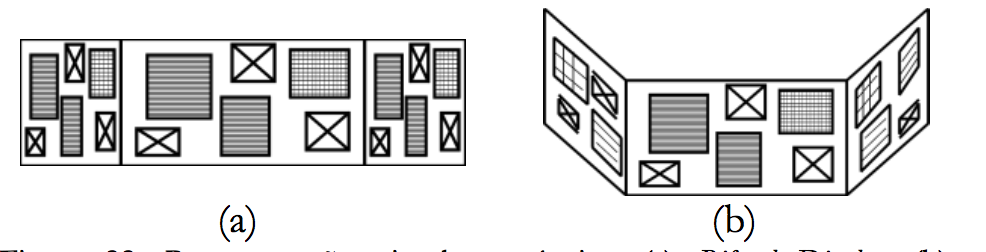
\includegraphics[scale=0.5]{Bifocal_Wall}
\caption{Comparativo entre a)Bifocal Display e b) Perspective Wall}
\label{img:comparativo}
\end{figure}
%
\end{itemize}
Uma revisão sistemática feita com foco em visualização de software \cite{salameh_software_2016} apresenta alguns questionamentos levantados pelos autores referente ao objetivo de se utilizar a técnica. As respostas encontradas pelos autores estavam divididas em quatro categorias. A primeira categoria encontrada baseava-se no artefato, a técnica era utilizada para acompanhar a evolução dos artefatos no repositório ao longo do tempo. A segunda categoria estava focada nas métricas, o objetivo estava em observar a alteração das métricas ao passar das entregas. A terceira categoria estava voltada para \textit{features}, o acompanhamento focava em analisar como e quais \textit{features} mudavam ao longo do tempo. A última categoria era centrada na arquitetura e em perceber as mudanças que estão envolvidas. Este trabalho tem seu objetivo focado na segunda categoria, acompanhar as métricas ao longo de um período de tempo e exibir para o usuário.
\\Para que se possa acompanhar as métricas dos projetos é necessário que se mantenha um histórico das métricas coletadas em momentos diferentes do desenvolvimento do software para que seja possível fazer uma comparação \cite{da_silva_iavems:_2010}. Em seus estudos \cite{gracanin_software_2005} aponta três características que são necessárias para que se faça um bom acompanhamento histórico do software.
\begin{itemize}
\item \textbf{Tempo}: A visualização deve ser agrupada através do número da release ou outro indicador que possua um tempo definido. Deve ser feito um \textit{snapshot} do sistema em que é possível ver claramente quais alterações foram realizadas.
\item \textbf{Estrutura}: O sistema deve ser decomposto em sub-sistemas, cada sub-sistema decomposto em módulos e cada módulo responsável por uma parte do código.
\item \textbf{Atributos}: Deve conter o número da versão, tamanho, alterações, complexidade.
\end{itemize}

Uma vez que é coletado os dados, eles ja estão categorizados de acordo com a sua natureza e ja podem ser exibidos ainda é necessário discutir qual a melhor forma de exibir todas essas informações na tela. Uma das formas de se agrupar toda a informação de maneira ordenada e com sentido lógico é através de \textit{dashboards}. O conceito será apresentado no tópico a seguir.

\subsection{Dashboard}
O conceito apresentado por Stephen Few em seu livro \cite{book_design} diz que um \textit{dashboard} é um \textit{display} virtual das informações mais importantes para atingir um ou mais objetivos, ele deve ser construido e organizado para ser capaz de caber em uma única página para que a informação seja achada com facilidade.